% Provenance (never printed): see sources/outline_sources.md and sources/book1/BRIEFS.md (g9/06).
\chapter{Secret Codes: A First Look at Cryptography}\label{ch:g9:first-cryptography}

Lina and Sami pass notes in class. To keep them private, they replace every
letter by the one three places further in the alphabet: \texttt{see you at
noon} becomes \texttt{vhh brx dw qrrq}. One day their teacher picks up a note,
looks at it for a minute, and reads it out loud. How did she do it, and how
could they have done better? This chapter writes secret codes in Python, and
then breaks them.

\begin{recall}
A \omterm{def:g7:strings:string}{string} is a sequence of \omterm{def:g7:strings:string}{characters}; \code{ord} gives the code of a \omterm{def:g7:strings:string}{character}
and \code{chr} the \omterm{def:g7:strings:string}{character} of a code (\cref{ch:g7:strings}). A \omterm{def:g8:dictionaries:dictionary}{dictionary} can
count how often each \omterm{def:g6:variables-and-input:value}{value} appears (\cref{ch:g8:dictionaries}).
\code{random.shuffle} mixes a \omterm{def:g7:lists:list}{list}, and a \omterm{def:g9:randomness-and-simulation:seed}{seed} makes it repeat
(\cref{ch:g9:randomness-and-simulation}). A \omterm{def:g5:networks-first-look:password}{password} proves who you are to a
\omterm{def:g5:networks-first-look:server}{server} (\cref{ch:g5:networks-first-look}).
\end{recall}

\section{Encrypting and decrypting with a key}

\begin{definition}[Cipher, plaintext, ciphertext]\label{def:g9:first-cryptography:cipher}
A \emph{cipher}\index{cipher} is a method that turns a readable message, the
\emph{plaintext}\index{plaintext}, into a scrambled one, the
\emph{ciphertext}\index{ciphertext}, and back.
\end{definition}

\begin{definition}[Encryption and decryption]\label{def:g9:first-cryptography:encryption}
\emph{Encryption}\index{encryption} turns \omterm{def:g9:first-cryptography:cipher}{plaintext} into \omterm{def:g9:first-cryptography:cipher}{ciphertext};
\emph{decryption}\index{decryption} turns the \omterm{def:g9:first-cryptography:cipher}{ciphertext} back into the
\omterm{def:g9:first-cryptography:cipher}{plaintext}.
\end{definition}

\begin{definition}[Encryption key]\label{def:g9:first-cryptography:key}
The \emph{encryption key}\index{encryption key} of a \omterm{def:g9:first-cryptography:cipher}{cipher} is the secret
setting that the sender and the receiver share, such as the number of places
each letter moves. The same \omterm{def:g9:first-cryptography:cipher}{cipher} with another key gives another \omterm{def:g9:first-cryptography:cipher}{ciphertext}.
\end{definition}

The \omterm{def:g9:first-cryptography:cipher}{ciphertext} travels where anyone may see it: on a note passed across the
room, or over a \omterm{def:g5:networks-first-look:network}{network}. The method is often known to all; only the key is
secret. A good \omterm{def:g9:first-cryptography:cipher}{cipher} stays safe even when the enemy knows how it works, as
long as the key stays hidden.

\begin{omfigure}
\begin{tikzpicture}[box/.style={draw=ocInk, rounded corners=2pt, fill=ocBlue!12,
    minimum height=8mm, align=center, font=\small}]
  \node[box] (s) at (0,0) {Lina\\ plaintext};
  \node[box, fill=ocYellow!40] (e) at (2.9,0) {encrypt};
  \node[box, fill=ocYellow!40] (d) at (8.3,0) {decrypt};
  \node[box] (r) at (11.2,0) {Sami\\ plaintext};
  \draw[-{Stealth}] (s) -- (e);
  \draw[-{Stealth}, ocRed, thick] (e) -- node[above, font=\small\ttfamily] {vhh brx dw qrrq}
    node[below, font=\scriptsize, black!60] {ciphertext, seen by anyone} (d);
  \draw[-{Stealth}] (d) -- (r);
  \node[box, fill=ocMint!40] (k1) at (2.9,1.5) {key 3};
  \node[box, fill=ocMint!40] (k2) at (8.3,1.5) {key 3};
  \draw[-{Stealth}] (k1) -- (e);
  \draw[-{Stealth}] (k2) -- (d);
  \node[box, fill=black!8] (t) at (5.6,-2.0) {someone listening:\\ no key};
  \draw[-{Stealth}, dashed] (5.6,-0.5) -- (t);
\end{tikzpicture}

{\small A secret message: the key is shared in advance; the \omterm{def:g9:first-cryptography:cipher}{ciphertext} travels in
the open, where someone without the key can read it but should not understand
it.}
\end{omfigure}

\section{The shift cipher and its 25 keys}

\begin{definition}[Shift cipher]\label{def:g9:first-cryptography:shift-cipher}
A \emph{shift cipher}\index{shift cipher} moves every letter of the \omterm{def:g9:first-cryptography:cipher}{plaintext}
the same number of places along the alphabet, going round from z back to a. The
number of places is the key.
\end{definition}

\begin{omfigure}
\begin{tikzpicture}
  \foreach \l/\c [count=\i from 0] in {a/D, b/E, c/F, d/G, e/H, f/I, g/J, h/K, i/L, j/M, k/N, l/O, m/P, n/Q, o/R, p/S, q/T, r/U, s/V, t/W, u/X, v/Y, w/Z, x/A, y/B, z/C} {
    \node[font=\small\ttfamily] at ({90 - \i * 360/26}:2.75cm) {\l};
    \node[font=\small\ttfamily\bfseries, ocRed] at ({90 - \i * 360/26}:2.05cm) {\c};
  }
  \draw[black!40] (0,0) circle (3.1cm) (0,0) circle (2.4cm) (0,0) circle (1.7cm);
  \node[align=center, font=\small] at (0,0) {outer: plaintext\\ inner: ciphertext\\ shift 3};
\end{tikzpicture}

{\small A \omterm{def:g9:first-cryptography:cipher}{cipher} wheel set to shift 3: each letter of the outer ring is replaced
by the letter just inside it (a by D, b by E, \ldots, x by A).}
\end{omfigure}

% ledger: g9:caesar-shift
This \omterm{def:g9:first-cryptography:cipher}{cipher} is very old. A Roman historian wrote that Julius Caesar used it for
his confidential letters: to read them, one had to put D for A, and so on with
the other letters, a shift of three.

In Python, a letter's position in the alphabet is \code{ord(letter) - ord("a")},
from 0 to 25. Adding the key and keeping the remainder by 26 makes the
alphabet go round:

\omcode{code/grade-9/06-first-cryptography/listings/shift.py}{1}{21}{The \omterm{def:g9:first-cryptography:shift-cipher}{shift
cipher}.}\label{lst:g9:first-cryptography:shift}

\Needspace*{6\baselineskip}
\omoutput{code/grade-9/06-first-cryptography/outputs/shift.txt}{x, y and z go round
to a, b and c.}\label{out:g9:first-cryptography:shift}

To decrypt, shift by the opposite of the key. Python's \texttt{\%} keeps the
result between 0 and 25 even when the number is negative:

\Needspace*{8\baselineskip}
\omcode{code/grade-9/06-first-cryptography/listings/shift_back.py}{1}{5}{Decrypting:
the same \omterm{def:g7:functions:function}{function}, the opposite key.}\label{lst:g9:first-cryptography:back}

\Needspace*{6\baselineskip}
\omoutput{code/grade-9/06-first-cryptography/outputs/shift_back.txt}{There and
back.}\label{out:g9:first-cryptography:back}

\begin{definition}[Brute-force search]\label{def:g9:first-cryptography:brute-force}
A \emph{brute-force search}\index{brute-force search} tries every possible key,
one after the other, until one gives a readable message.
\end{definition}

The \omterm{def:g9:first-cryptography:shift-cipher}{shift cipher} has only 25 useful keys, so a \omterm{def:g4:programs-and-operating-system:program}{program} tries them all in a
blink:

\Needspace*{8\baselineskip}
\omcode{code/grade-9/06-first-cryptography/listings/brute_force.py}{1}{5}{Every
key, one after the other.}\label{lst:g9:first-cryptography:brute}

\omoutput[1-15]{code/grade-9/06-first-cryptography/outputs/brute_force.txt}{Key 13
gives English.}\label{out:g9:first-cryptography:brute}

That is how the teacher read Lina's note: a person can try 25 shifts by hand in
a few minutes. A \omterm{def:g9:first-cryptography:cipher}{cipher} is only as strong as the work it takes to try all its
keys.

\begin{omfigure}
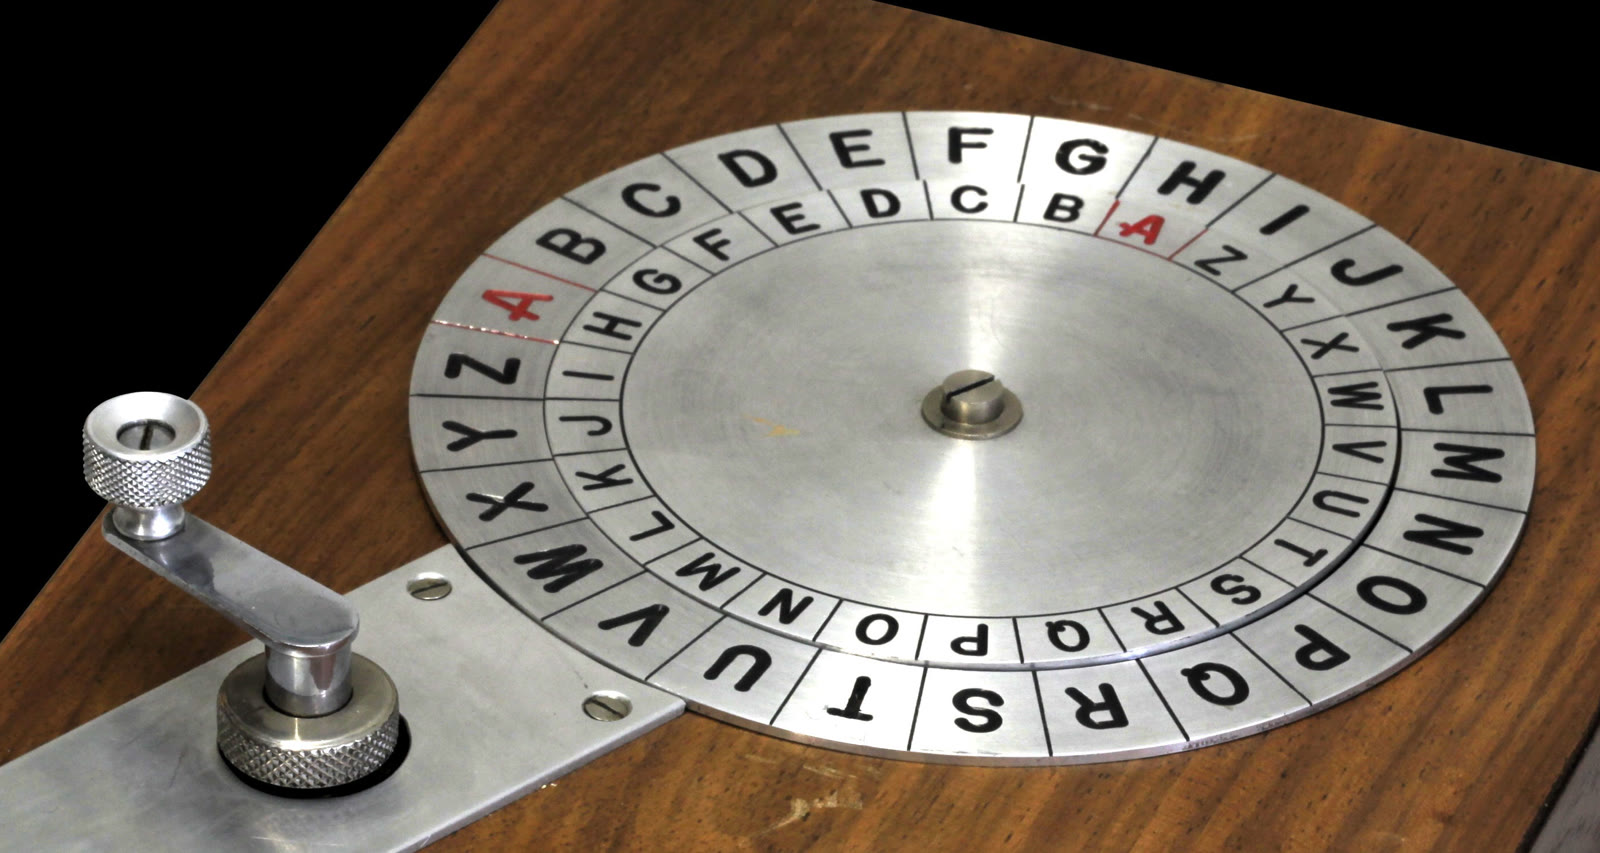
\includegraphics[width=0.6\linewidth]{images/book1/g9-cipher-wheel.jpg}

{\small A \omterm{def:g9:first-cryptography:cipher}{cipher} wheel once used to train soldiers: the inner ring turns
against the outer one, and the position chosen is the key. On this wheel the
inner alphabet runs the other way round.}
\end{omfigure}

\section{Substitution ciphers and letter frequencies}

\begin{definition}[Substitution cipher]\label{def:g9:first-cryptography:substitution-cipher}
A \emph{substitution cipher}\index{substitution cipher} replaces each letter by
another, following a table in which every letter of the alphabet appears once:
the key is a mixed alphabet.
\end{definition}

The \omterm{def:g9:first-cryptography:shift-cipher}{shift cipher} is the special case where the table is the alphabet turned
round. A general key is any shuffle of the alphabet:

\omcode{code/grade-9/06-first-cryptography/listings/substitution.py}{1}{31}{A
\omterm{def:g9:first-cryptography:substitution-cipher}{substitution cipher} with a shuffled alphabet.}\label{lst:g9:first-cryptography:substitution}

\Needspace*{8\baselineskip}
\omoutput{code/grade-9/06-first-cryptography/outputs/substitution.txt}{The key
replaces a by m, b by i, and so on.}\label{out:g9:first-cryptography:substitution}

How many keys are there? 26 choices for the letter that replaces a, then 25 for
b, 24 for c, and so on down to 1:

\Needspace*{7\baselineskip}
\omcode{code/grade-9/06-first-cryptography/listings/count_keys.py}{1}{4}{Counting
the keys.}\label{lst:g9:first-cryptography:count}

\Needspace*{5\baselineskip}
\omoutput{code/grade-9/06-first-cryptography/outputs/count_keys.txt}{A 27-digit
number.}\label{out:g9:first-cryptography:count}

Far too many to try, even for a \omterm{def:g1:what-is-a-computer:computer}{computer}
(Exercise~\ref{exo:g9:first-cryptography:10}). But the \omterm{def:g9:first-cryptography:cipher}{cipher} has a weakness:
each letter is always replaced by the same symbol, so the \omterm{def:g9:first-cryptography:cipher}{ciphertext} keeps the
letter frequencies of the language.

\begin{definition}[Frequency analysis]\label{def:g9:first-cryptography:frequency-analysis}
\emph{Frequency analysis}\index{frequency analysis} breaks a \omterm{def:g9:first-cryptography:substitution-cipher}{substitution cipher}
by counting how often each symbol appears in the \omterm{def:g9:first-cryptography:cipher}{ciphertext} and matching the
most frequent symbols with the most frequent letters of the language.
\end{definition}

The chapter keeps an invented passage of four paragraphs in a \omterm{def:g8:files-and-data-tables:text-file}{text file},
\code{passage.txt}. It begins:

\Needspace*{6\baselineskip}
\omcode{code/grade-9/06-first-cryptography/listings/passage.txt}{1}{3}{The first lines
of the chapter's passage.}\label{lst:g9:first-cryptography:passage}

Counting its letters with a \omterm{def:g8:dictionaries:dictionary}{dictionary}:

\omcode{code/grade-9/06-first-cryptography/listings/frequencies.py}{1}{22}{The
letters of the passage, the most frequent first.}\label{lst:g9:first-cryptography:frequencies}

\omoutput{code/grade-9/06-first-cryptography/outputs/frequencies.txt}{E, t, h and a
lead.}\label{out:g9:first-cryptography:frequencies}

\code{sorted} with \code{key=lambda letter: -counts[letter]} sorts the letters by
their counts, largest first: a \code{lambda} is a \omterm{def:g7:functions:function}{function} written in one line,
here ``given a letter, return minus its count''.

\begin{omfigure}
\begin{tikzpicture}
  \foreach \col/\title/\colour [count=\n from 0] in {plain/plaintext/ocBlue, cipher/ciphertext (shift 3)/ocRed} {
    \begin{axis}[at={(0,-\n*4.1cm)}, width=13cm, height=4cm, ybar, bar width=2.6mm,
        ymin=0, ymax=230, xtick=data, symbolic x coords={a,b,c,d,e,f,g,h,i,j,k,l,m,n,o,p,q,r,s,t,u,v,w,x,y,z},
        x tick label style={font=\small\ttfamily}, enlarge x limits=0.03,
        ylabel={count}, title={\small \title}]
      \addplot[fill=\colour!60, draw=\colour] table[x=letter, y=\col]
        {code/grade-9/06-first-cryptography/figures/out/letters.dat};
    \end{axis}
  }
\end{tikzpicture}

{\small The letter counts of the passage and of its \omterm{def:g9:first-cryptography:cipher}{ciphertext} with shift 3: the
same bars, moved three places to the right. The tallest bar, e, has become h.}
\end{omfigure}

The same works on a \omterm{def:g9:first-cryptography:substitution-cipher}{substitution cipher}, with a long text in the same
language as a guide. The \omterm{def:g4:programs-and-operating-system:program}{program} below takes the first two paragraphs of the
passage as the known text, encrypts the last two with a random key, and guesses
the key by matching the letters in order of frequency:

\omcode{code/grade-9/06-first-cryptography/listings/guess_substitution.py}{1}{33}{A
first guess from frequencies, then two corrections.}\label{lst:g9:first-cryptography:guess}

\Needspace*{10\baselineskip}
\omoutput{code/grade-9/06-first-cryptography/outputs/guess_substitution.txt}{Each line
shows the start of the guessed message and the number of letters
right.}\label{out:g9:first-cryptography:guess}

The first guess already gets \code{the} right, and about half of the letters.
The rest comes from reading: \code{pheo the eveosou} looks like
\code{when the evening}, so o and n swap; then \code{trdab} looks like
\code{today}, so r and o swap. Each correction gets more letters right, from
401 to 453 to 514 of the 810; a few more of the same kind make the whole
message clear.

\begin{history}[Counting letters]
% ledger: g9:al-kindi
% ledger: g9:polyalphabetic
In the ninth century, in Baghdad, the scholar al-Kindi wrote a manuscript on
deciphering secret messages. His method: take a fairly long text in the same
language, count each of its letters, and rank them; then rank the symbols of
the secret message the same way, and match first with first, second with
second. His own counts used seven pages, 3,667 letters. Much later, in Europe,
writers on \omterm{def:g9:first-cryptography:cipher}{ciphers} such as Alberti, Bellaso and Vigenère described \omterm{def:g9:first-cryptography:cipher}{ciphers} that
change the shift from letter to letter, against this kind of attack.
\end{history}

\section{A cipher with a keyword}

\begin{definition}[Keyword cipher]\label{def:g9:first-cryptography:keyword-cipher}
A \emph{keyword cipher}\index{keyword cipher} shifts each letter of the \omterm{def:g9:first-cryptography:cipher}{plaintext}
by a different amount, given in turn by the letters of a keyword (a for 0, b for
1, and so on); after the last letter of the keyword, it starts again from the
first.
\end{definition}

\begin{omfigure}
\begin{tikzpicture}[x=0.62cm, y=0.62cm]
  \foreach \p/\k/\s/\c [count=\i from 0] in {m/l/11/x, e/a/0/e, e/m/12/q, t/p/15/i, m/l/11/x, e/a/0/e, a/m/12/m, t/p/15/i} {
    \node[font=\ttfamily] at (\i*1.6,2) {\p};
    \node[font=\ttfamily, ocBlue] at (\i*1.6,1) {\k};
    \node[font=\scriptsize, black!60] at (\i*1.6,0.1) {+\s};
    \node[font=\ttfamily\bfseries, ocRed] at (\i*1.6,-0.9) {\c};
  }
  \node[anchor=east, font=\small] at (-0.8,2) {plaintext};
  \node[anchor=east, font=\small, ocBlue] at (-0.8,1) {keyword};
  \node[anchor=east, font=\small] at (-0.8,0.1) {shift};
  \node[anchor=east, font=\small, ocRed] at (-0.8,-0.9) {ciphertext};
\end{tikzpicture}

{\small The keyword \texttt{lamp} over \texttt{meet me at}: each letter moves by
the keyword letter above it (l = 11, a = 0, m = 12, p = 15). The two e's of
\texttt{meet} become e and q, and the two m's both become x, because they fall
under the same keyword letter.}
\end{omfigure}

\omcode{code/grade-9/06-first-cryptography/listings/keyword_cipher.py}{1}{19}{The
\omterm{def:g9:first-cryptography:keyword-cipher}{keyword cipher}.}\label{lst:g9:first-cryptography:keyword}

\Needspace*{5\baselineskip}
\omoutput{code/grade-9/06-first-cryptography/outputs/keyword_cipher.txt}{The message
with the keyword lamp.}\label{out:g9:first-cryptography:keyword}

The \omterm{def:g6:while-loops:counter}{counter} \code{k} moves only on letters, so spaces do not use up keyword
letters. A same \omterm{def:g9:first-cryptography:cipher}{plaintext} letter now gives several \omterm{def:g9:first-cryptography:cipher}{ciphertext} letters, and the
frequencies flatten:

\omcode{code/grade-9/06-first-cryptography/listings/keyword_frequencies.py}{1}{18}{The
four most frequent letters, with three \omterm{def:g9:first-cryptography:cipher}{ciphers}.}\label{lst:g9:first-cryptography:keyfreq}

\Needspace*{8\baselineskip}
\omoutput{code/grade-9/06-first-cryptography/outputs/keyword_frequencies.txt}{The
longer the keyword, the flatter the counts.}\label{out:g9:first-cryptography:keyfreq}

The \omterm{def:g9:first-cryptography:shift-cipher}{shift cipher} keeps the exact counts, just on other letters. With the
four-letter keyword, the top letter falls from 14.0\,\% to 10.3\,\%; with the
ten-letter keyword \code{lighthouse}, to 6.3\,\%, and the top four are nearly
level. A longer keyword spreads each letter over more shifts. It can still be
broken: each fourth letter is shifted the same way, and repeated groups of
letters betray the keyword's length (Exercise~\ref{exo:g9:first-cryptography:12}).

\section{Why a long random key resists; the padlock in a browser}

Every \omterm{def:g9:first-cryptography:cipher}{cipher} of this chapter is broken by a pattern that the key leaves in the
\omterm{def:g9:first-cryptography:cipher}{ciphertext}. Take that idea to its end: a keyword as long as the message itself,
its letters chosen at random (with a generator made for secrets, not
\code{random}), and never used twice. Then every shift is independent of the
others, every \omterm{def:g9:first-cryptography:cipher}{plaintext} of that length is equally possible, and no counting can
help. The price is a key as long as everything one wants to send, shared in
advance.

When the address bar of a \omterm{def:g5:networks-first-look:page}{browser} shows a padlock, the page travels between the
\omterm{def:g5:networks-first-look:server}{server} and your \omterm{def:g1:what-is-a-computer:computer}{computer} encrypted, and the \omterm{def:g5:networks-first-look:server}{server} has proved its name, so that
another machine cannot pretend to be it. The \omterm{def:g9:first-cryptography:cipher}{ciphers} used there are far
stronger than those of this chapter, and the two \omterm{def:g1:what-is-a-computer:computer}{computers} agree on a fresh key
without ever sending it in the open. How they do it is told in the next book.

\section{Exercises}

\begin{exercise}[$\star$]\label{exo:g9:first-cryptography:1}
Encrypt \code{code} with the \omterm{def:g9:first-cryptography:shift-cipher}{shift cipher} and the key 3.
\end{exercise}

\begin{exercise}[$\star$]\label{exo:g9:first-cryptography:2}
The word \code{qeb} was encrypted with the key 23. Decrypt it.
\end{exercise}

\begin{exercise}[$\star$]\label{exo:g9:first-cryptography:3}
What does \code{count_keys.py} compute, step by step, for an alphabet of only
4 letters? How many substitution keys does such an alphabet have?
\end{exercise}

\begin{exercise}[$\star$]\label{exo:g9:first-cryptography:4}
Write a \omterm{def:g9:first-cryptography:shift-cipher}{shift cipher} that keeps capital letters as capitals and leaves spaces,
punctuation and digits unchanged. Try it on \code{Meet Me at Noon, by the Zoo!}
with the key 3.
\end{exercise}

\begin{exercise}[$\star\star$]\label{exo:g9:first-cryptography:5}
This \omterm{def:g7:functions:function}{function} forgets the alphabet's end. What does it print? Fix it.

\omcode{code/grade-9/06-first-cryptography/exercises/shift_bug.py}{1}{5}{A shift
without the remainder.}\label{lst:g9:first-cryptography:shift-bug}
\end{exercise}

\begin{exercise}[$\star\star$]\label{exo:g9:first-cryptography:6}
This \omterm{def:g4:programs-and-operating-system:program}{program} should print the message back. What does it print instead, and
why? Fix it.

\omcode{code/grade-9/06-first-cryptography/exercises/decrypt_bug.py}{1}{4}{A
\omterm{def:g9:first-cryptography:encryption}{decryption}.}\label{lst:g9:first-cryptography:decrypt-bug}
\end{exercise}

\begin{exercise}[$\star\star$]\label{exo:g9:first-cryptography:7}
Write a \omterm{def:g9:first-cryptography:brute-force}{brute-force search} that prints only the \omterm{def:g9:first-cryptography:encryption}{decryption} with the most common
English words (\code{the}, \code{and}, \code{a}, \code{to}, \code{of},
\code{in}, \code{at}, \code{is}, \code{it}, \code{on}). Try it on
\code{vjg mggrgt nkv vjg ncor cv vjg gpf qh vjg fca}.
\end{exercise}

\begin{exercise}[$\star\star$]\label{exo:g9:first-cryptography:8}
Write \code{keyword_decrypt(text, keyword)}, which undoes the \omterm{def:g9:first-cryptography:keyword-cipher}{keyword cipher},
and check it on the \omterm{def:g9:first-cryptography:cipher}{ciphertext} of \cref{out:g9:first-cryptography:keyword}.
\end{exercise}

\begin{exercise}[$\star\star$]\label{exo:g9:first-cryptography:9}
What does a shift of 26 do to a message? And a shift of 29? Why does the \omterm{def:g9:first-cryptography:shift-cipher}{shift
cipher} have 25 useful keys and not 26 or more?
\end{exercise}

\begin{exercise}[$\star\star\star$]\label{exo:g9:first-cryptography:10}
A \omterm{def:g1:what-is-a-computer:computer}{computer} tries a billion substitution keys per second. How many years does it
need to try them all? Compute it with a \omterm{def:g4:programs-and-operating-system:program}{program}.
\end{exercise}

\begin{exercise}[$\star\star\star$]\label{exo:g9:first-cryptography:11}
Count the five most frequent letters in the first 20, 100 and 1,000 letters of
the passage, with a \omterm{def:g4:programs-and-operating-system:program}{program}. Use the counts to explain why \omterm{def:g9:first-cryptography:frequency-analysis}{frequency analysis}
needs a long \omterm{def:g9:first-cryptography:cipher}{ciphertext}.
\end{exercise}

\begin{exercise}[$\star\star\star$]\label{exo:g9:first-cryptography:12}
The passage, without spaces, is encrypted with the keyword \code{lamp}. Write a
\omterm{def:g4:programs-and-operating-system:program}{program} that finds every group of three letters that appears again later in the
\omterm{def:g9:first-cryptography:cipher}{ciphertext}, and records the distance between the two places. Then count, for
each length from 2 to 8, how many distances it divides. Which length stands
out, and why?
\end{exercise}

\section{Problem: Breaking a Message without the Key}

\begin{problem}[{Weekend problem --- breaking a message without the key}]\label{pb:g9:first-cryptography:1}
A message from the passage has been encrypted with the \omterm{def:g9:first-cryptography:shift-cipher}{shift cipher} and an
unknown key. Can a \omterm{def:g4:programs-and-operating-system:program}{program} find the key with no help but letter counts? And how
long must the message be?

\needspace{4\baselineskip}\medskip\noindent\textbf{Part I --- By hand.}

\omcode{code/grade-9/06-first-cryptography/listings/guess_shift.py}{1}{19}{Guessing
a shift key from the most frequent letter.}\label{lst:g9:first-cryptography:guess-shift}

\omoutput[1-2]{code/grade-9/06-first-cryptography/outputs/guess_shift.txt}{The first
line of the \omterm{def:g9:first-cryptography:cipher}{ciphertext}.}\label{out:g9:first-cryptography:cipher-line}

\begin{enumerate}
  \item Count the letters of this line by hand. Which letter is the most frequent?
  \item If that letter stands for e, what is the key?
  \item Decrypt the first word with that key. Does it make sense? If not, try
    the second most frequent letter.
\end{enumerate}

\needspace{4\baselineskip}\medskip\noindent\textbf{Part II --- A program guesses.}
\begin{enumerate}[resume]
  \item What does \code{guess_key} assume, and how does it turn the most frequent
    letter into a key?
  \item Why is the result taken modulo 26?
  \item Run the \omterm{def:g4:programs-and-operating-system:program}{program}. Does it find the key, and is the whole message right?
  \item On which kind of message would this guess fail, even if it were long?
\end{enumerate}

\needspace{4\baselineskip}\medskip\noindent\textbf{Part III --- How long must the message be?}

\omcode{code/grade-9/06-first-cryptography/listings/short_messages.py}{1}{21}{Guessing
the key of 100 messages of each length.}\label{lst:g9:first-cryptography:short}

\begin{enumerate}[resume]
  \item Where do the 100 messages of each length come from, and with which keys
    are they encrypted?
  \item Run it. How often is the key found with 10 letters? With 100?
  \item Why is 200 letters barely better than 100, and 500 letters perfect?
  \item What does this tell Lina and Sami about short notes?
  \item State the result.
\end{enumerate}
\end{problem}
